% !TeX root = ../Bachelorarbeit.tex
\chapter{Grundlagen}
Laut des IT-Grundschutz-Kompendiums vom \ac{bsi} könne ein Benutzer aus Bequemlichkeit oder pragmatischen Gründen bewusst auf komplizierte und unhandliche Kryptomodule verzichten und Informationen stattdessen im Klartext übertragen. \cite{A5} Dies stellt ein hohes Sicherheitsrisiko für Unternehmen, aber auch Privatpersonen dar, da Benutzer nicht gewillt sind ihre Passwörter durch komplizierte Verfahren zu erzeugen und in regelmäßigen Abständen vollkommen randomisiert zu setzen. An neuartige Ansätze des Logins in nativen oder webbasierten Anwendungen stellen sich dadurch völlig neue Herausforderungen. So müssen neue Authentifizierungsmöglichkeiten nicht nur sicher sein, sondern auch komfortabel genutzt und bedient werden können, da sie sonst von den Endnutzern gemieden oder umgangen werden. Wichtig ist auch, dass die breite Masse Zugriff auf die Ressourcen hat, die es zur Nutzung dieser Verfahren braucht. Man denke nur an die ganzen betrieblichen Passwörter, bei denen zum Monatsende nur eine Zahl an der letzten Stelle des Passwortes geändert wird. Laut einer Statistik von 2019, der ``Global Data Risk Report From the Varonis Data Lab'', gaben 38\% aller Nutzer an ein Passwort im Unternehmen zu nutzen, das sie nicht (oder nur geringfügig) ändern. Außerdem wird laut dieser Statistik alle 364 Tage wahrscheinlich ein Data Breach aufgrund von unsicheren Passwörtern in einem mittelständigen Unternehmen stattfinden. Die monatliche Ablaufzeit von Passwörtern in Unternehmen scheint also nicht ganz den Effekt zu erzielen, der ursprünglich damit geplant war, da die Arbeiter die Bequemlichkeit über die Sicherheit stellen.

\section{IT-Grundschutzkriterien}
Der IT-Grundschutz definiert den Schutzbedarf eines bestimmten Assets je nachdem welches Risiko bei Verletzung der Grundwerte Vertraulichkeit, Integrität und Verfügbarkeit entstehen \cite{A7}.
\newpage

Der \ac{bsi} spezifiziert folgende Schutzbedarfskategorien:
\begin{itemize} 
\item \textbf{normal} (Schadenauswirkungen begrenzt bis überschaubar)
\item \textbf{hoch} (Schadenauswirkungen könnten hoch bzw. beträchtlich sein)
\item \textbf{sehr hoch} (Schadensauswirkungen können ein existenziell bedrohliches Ausmaß annehmen
\end{itemize}
Bei dem Authentifikationsprototypen wird die Schadensauswirkung für alle nicht personenbezogenen Daten wohl im Bereich normal liegen, da schon im Aufbau darauf geachtet wird, dass nur so viele Daten vom User verwendet werden, wie zwingend notwendig. (Nach dem Need-To-Know Prinzip) Sollte die Webseite oder Teile der Webseite publiziert bzw. im Business - Umfeld genutzt werden, muss eine Neubewertung der Daten nach Vertraulichkeit, Integrität und Verfügbarkeit stattfinden. Vor allem muss darauf geachtet werden, dass Daten über Fingerabdrücke verschlüsselt und Passwörter im gehashten Zustand in Datenbanken persistiert sind.

Gleichzeitig sollten die genutzten Verfahren insgesamt mathematisch sicher sein, auf veraltete Verschlüsselungsverfahren ist zu verzichten. Dies gilt auch für Hashverfahren wie MD5, die häufig durch sehr große vorgerechnete Tabellen erraten werden können. Stattdessen ist auf Verfahren wie SHA512 (Gehasht mit Salt und Pepper) zu setzen.

Bei Kompromittierung des Servers, welches die größte Bedrohung für den Prototypen darstellt, droht ein Data-Breach. Dies kann für ein Unternehmen einen Imageschaden sowie weitreichende juristische Klagen zur Folge haben. Das sind bereits 2 der 7 aufgeführten Schadensszenarien durch den \ac{bsi}, wobei einer bereits eine Zertifizierung begründen kann. Je nach dem wie kompliziert die Ursprungsdaten sind und welcher Hashingalgorithmus in Kombination mit Salt und Pepper genutzt wurde, können vorallem Nutzerpassphrasen an die Öffentlichkeit gelangen und Angreifer können die Passwörter für andere Dienste nutzen. Dies setzt voraus, dass ein Angreifer an den Hash des Passwortes kommt und den Pepper des Servers auslesen kann. Und anschließend mit dem Salt des Nutzers und dem Pepper des Servers das Passwort errechnet durch Bruteforce. Die Wahrscheinlichkeit für diesen Schaden ist sehr niedrig (Schadenskategorie normal).
\newpage

\begin{figure}[ht]
	\centering
	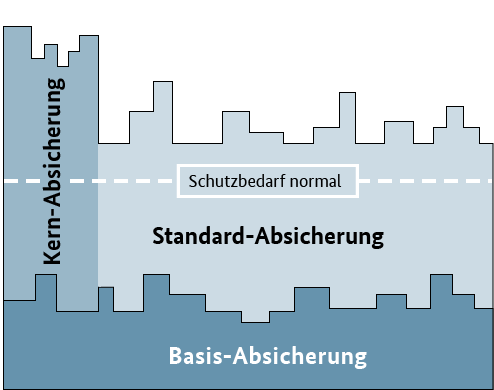
\includegraphics [width=13cm]{Abb_2_09_Varianten.png}
	\caption[Absicherungsarten nach \ac{bsi} und IT-Grundschutz]{Absicherungsarten nach \ac{bsi} und IT-Grundschutz}
	\label{fig:Abb_2_09_Varianten}
\end{figure}

Der IT-Grundschutz beschreibt die drei Arten der Absicherung wie folgt. Die Basis-Absicherung ist relevant für Institutionen die einen Einstieg in den IT-Grundschutz suchen und relativ schnell alle relevanten Geschäftspozesse mit einfach umzusetzenden Basismaßnahmen sichern wollen. Die Kern-Absicherung konzentriert sich auf besonders wichtige Geschäftsprozesse und vertieft sich in die Sicherung dieser. Von einer Standard-Absicherung spricht man, wenn alle empfohlenen IT-Grundschutz-Vorgehensweisen durchgeführt werden. Sie beschreibt den allumfassenden Schutz der Prozesse und Bereiche der Institution, wie das Bild des \ac{bsi} verdeutlicht. \cite{A8}

Bei dem Prototyp wird eine Basis-Absicherung nach \ac{bsi} durchgeführt. Es wird darauf geachtet alle Datenschutzkriterien für Webanwendungen zu erfüllen. Kriterien die nicht erfüllt werden konnten oder wurden, werden dokumentiert und in der Auswertung erläutert. Die Wahl der Basis-Absicherung begründet sich damit, dass lokale Testdaten im Prototyp verarbeitet werden, für die kein bis nur ein sehr geringer Schutzbedarf besteht. Eine Kern-Absicherung käme nur in Frage, falls ein ganz bestimmter Prozess oder Asset des Prototyps geschützt werden müsste wie zum Beispiel der Zugriff auf die Datenbank durch den Prototypen. Insgesamt ist dieser Teil der Abschlussarbeit auch als Einstieg in den IT-Grundschutz zu verstehen, welcher laut \ac{bsi} selbst die Basis-Absicherung als Empfehlung und zur Folge hat und sich am Besten für vorhandene Zwecke eignet.

\section{Standard nach FIDO2}
Die genannten Probleme sind den Menschen seit einigen Jahren bekannt und wurden vor allem mit Verfahren gelöst, die keine Passwörter (oder allgemein Verfahren der Wissenskategorie) zur Authentifikation benötigen und diese maximal als ersten Layer der Sicherheit implementieren. Das bekannteste Beispiel für einen Standard zur sicheren und bequemen Authentifikation im Internet findet man unter dem Schlüsselwort FIDO2. FIDO steht dabei für 'Fast Identity Online' (Schnelle Identität im Netz). Sie ist das Ergebnis einer Kooperation des \ac{w3c} und der FIDO Alliance.


\begin{figure}[ht]
	\centering
	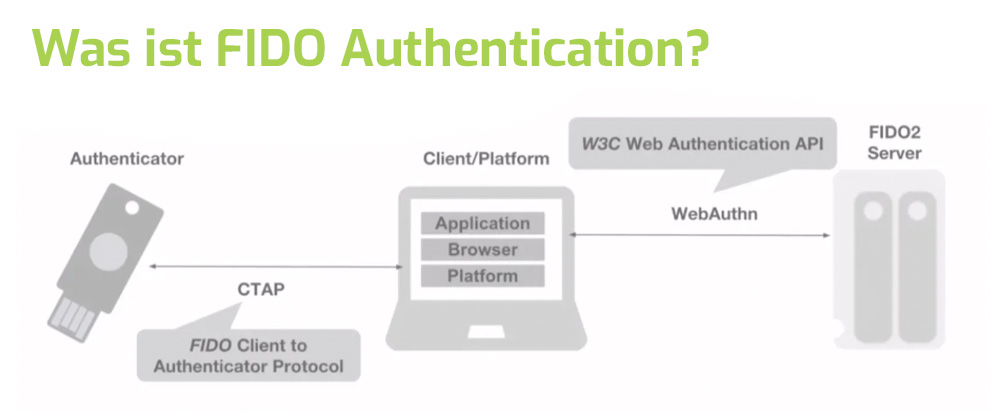
\includegraphics [width=15cm]{fido_authentication.jpg}
	\caption[Bestandteile der FIDO-Authentifikation]{Bestandteile der FIDO-Authentifikation}
	\label{fig:fido_authentication}
\end{figure}

Grundsätzlich besteht der Standard aus folgenden Komponenten:

\begin{itemize} 
\item \textbf{Authenticator}

Der Authenticator kann, wie im Schaubild von der offiziellen Seite der FIDO Alliance zur Frage 'Was ist die FIDO Authentifikation' bereits gezeigt, ein sogenannter ``FIDO2-USB'' sein. Also ein USB mit der Möglichkeit zur passwortlosen Authentifizierung des Nutzers im Netz. Eine weitere bekannte Möglichkeit für einen Authenticator ist Windows Hello (bestehend aus Hello-PIN, Hello-Fingerabdruck und Hello-Gesichtsmuster) oder Plat für Betriebssysteme vom Hersteller Apple.

So können also sowohl externe Geräte (mit eingebautem Schlüssel) sowie interne Geräte (sogenannte self-signed-devices, die selbst Schlüssel bei der Registration erzeugen) des Betriebssystems bzw. Rechners zur Authentifikation genutzt werden.
\newpage

\item \textbf{CTAP - Client to Authenticator Protocol}

Das \ac{ctap} bzw. genauer \ac{ctap}2 ist das Nachfolgeprotokoll zu \ac{u2f} welches mit der Einführung von FIDO2 in \ac{ctap}1 umbenannt wurde. Mit FIDO2 wurde die Kommunikation zwischen dem Authenticator und der Plattform (dem Browser, der Applikation) standardisiert. Das Protokoll definiert, dass der Server eine Initialanfrage an den User sendet. Dieser erstellt mittels des Authenticators ein Key-Pair, also einen öffentlichen und einen privaten Schlüssel und übermittelt den öffentlichen Schlüssel an den Server. Der Server persistiert diesen um zukünftige Anfragen des Nutzers zu identifizieren und den Nutzer zu authorisieren. Viele Schlüssel erfordern vor diesem Prozess eine Userverifikation, die zum externen Authenticator (dem USB - Stick) noch eine PIN verlangt, die beim Initiieren gesetzt wurde.

\item \textbf{Client/Platform}

Zwischen dem FIDO2-Server und dem Authenticator befindet sich der Client, hier interagiert der Nutzer mit dem Authenticator und verfiziert sich ihm Gegenüber. Über dessen Browser wird dann (über eine durch Webauthn erzwungene sichere Verbindung) ein Request an den FIDO2 - Server gestellt. Über den Client kommunizieren Server und Authenticator. Wichtig für alle diese Vorgänge ist, dass der private Schlüssel bei keiner Anfrage den Client verlässt. Er ist stets sicher auf dessen Rechner (im Trust Store unter Windows, je nach Betriebssystem variierend) lokalisiert.

\item \textbf{Webauthn}

Zwischen dem Server und der Plattform befindet sich das WebAuthn - Protokoll, welches in folgenden Kapiteln näher erläutert wird. Das Protokoll basiert auf zwei Hauptbestandteilen: Einem Registrier und einem künftigen Loginvorgang. Das Protokoll vermittelt dem Authenticator unter anderem die Optionen, die der Server für die Authentifikation erlaubt. So kann der Server zum Beispiel externe USB-Sticks verbieten oder eine ausdrückliche Authentifikation mittels NFC erzwingen. Wichtig ist, dass Webauthn keinerlei Details über den User freigibt. Ferner weiß weder der Server noch das Protokoll Webauthn welche der eigentlichen Authentifikationsmethoden vom User genutzt wurden. Webauthn gibt im ersten Schritt dem Nutzer die Optionen bei der Registration und kann im folgenden nur anhand des publicKey's und der credentialID erkennen, dass sich das Selbe gerät authorisieren möchte.

\item \textbf{FIDO2 - Server}

Ein FIDO2-Server ist ein durchschnittlischer Server auf dem typischerweise ein Javascript-Framework läuft, das als Backend für die Anfragen fungiert. Der Server verwaltet die öffentlichen Schlüssel des Nutzers und sorgt für die Verifikation der Anfragen für den Registrierungs und Loginprozess. Ferner wird bei sämtlichen Serverprozessen eine 'Relying Party Id' angegeben, welches die IP-Addresse des Servers ist. Teilweise findet man den Server in Abbildungen der FIDO - Alliance auch als 'Relying Party Server'. Erwähnt werden sollte allerdings, dass Client und Server sich die Authentifikation des Users bzw. die Logik hierzu teilen. Es findet im Vorhinein meist eine Userverifikation statt, bevor der Server über einen Loginversuch Kenntnis erlangt. Erst im Anschluss werden verschiedene Challenge-Response Anfragen zwischen Server und Client ausgetauscht.

\end{itemize}

\newpage

Unterschieden werden die einmalige Registrierung eines Gerätes für einen Nutzer und die folgende Authentifikation ('der Login') des Nutzers. Dessen Schritte werden im folgenden dargelegt.

\begin{figure}[ht]
	\centering
	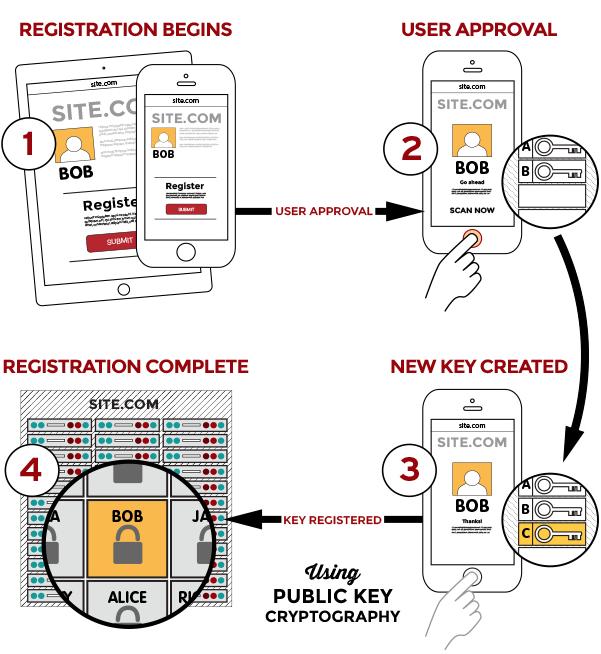
\includegraphics [width=9cm]{graphic_Registration.png}
	\caption[Userregistration nach FIDO2 mittels Webauthn \& CTAP2]{Userregistration nach FIDO2 mittels Webauthn \& CTAP2}
	\label{fig:graphic_Registration}
\end{figure}

\begin{enumerate}
 \item Der User wählt einen vom Server akzeptierten Authenticator aus. Hier ist es der Fingerabdruck. Auch möglich gewesen wäre ein gesprochenes Wort ins Mikrofon des Nutzers oder ein PIN sowie vieles mehr. Je nach Gerät (und Betriebssystem) können die möglichen Authentifizierungsmechanismen variieren.
 \item In der Phase der Userverifikation entsperrt der Nutzer den Authenticator durch seinen Fingerabdruck.
 \item Infolge dessen wird im dritten Schritt ein Paar aus privatem und öffentlichen Schlüssel erstellt. Der private Schlüssel bleibt auf dem Gerät des Endnutzers, während der öffentliche Schlüssel an den Server übermittelt wird.
 \item Dort wird dieser mit dem Useraccount verknüpft und persistiert um folgende Loginanfragen des Nutzers authentifizieren zu können. Der initiale Nutzer, der die Registrierung angestoßen hat, kann damit erkannt und effektiv authentisiert werden.
\end{enumerate}
\newpage

\begin{figure}[ht]
	\centering
	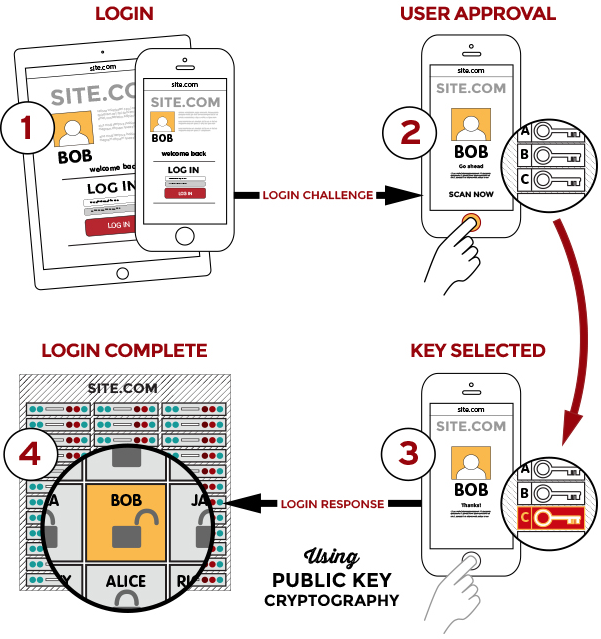
\includegraphics [width=9cm]{graphic_Login.png}
	\caption[Userauthentifikation nach FIDO2 mittels Webauthn \& CTAP2]{Userauthentifikation nach FIDO2 mittels Webauthn \& CTAP2}
	\label{fig:graphic_Registration}
\end{figure}

\begin{enumerate}
 \item Bei dem Loginvorgang wird der Nutzer dazu aufgefordert eine Challenge zu lösen.
 \item Die Geräteauswahlmöglichkeiten begrenzen sich hierbei auf Diejenige, die zuvor registriert wurden. Wenn der User also sowohl die PIN als auch die Gesichtserkennung eingerichtet hat, kann er sich zwischen den beiden Varianten entscheiden. Dieser Schritt ist identisch zum zweiten Schritt der Registration unter FIDO.
 \item Die Challenge des Servers wird mit dem privaten Schlüssel des Nutzers signiert und infolge dessen an den Server übermittelt.
 \item Der Server entschlüsselt diese mit dem gespeicherten öffentlichen Schlüssel aus der Registration. Der Nutzer erhält zum Ende der Authentifizierung eine zugehörige Response, die ihm den Login ermöglicht. Die Authentifikation des Nutzers ist damit abgeschlossen.
\end{enumerate}
\newpage

Zusammengefasst basiert FIDO2 auf vorhandenen Protokollen wie \ac{webauthn} für die Browser-Server-Kommunikation und \ac{ctap} für die Browser-Authenticator-Kommunikation. Die Yubico, einem der Hauptentwickler des heutigen \ac{ctap}1 - Protokolls, fasst FIDO2 wie folgt zusammen: ''an open authentication standard that enables internet users to securely access any number of online services with one single security key [...]. FIDO2 is the latest generation of the \ac{u2f} protocol`` [5] (übersetzt: Ein offener Authentifikationsstandard der Usern das Erreichen von Online-Services mittels eines einzigen sicheren Schlüssels erlaubt. [...] FIDO2 ist die letzte Generation des \ac{u2f} - Protokolls). Während das Vorgänger - Protokoll \ac{u2f} von Google und Yubico ins Leben gerufen wurde, ist FIDO2 ein offener dezentraler Kommunikationsstandart für die passwortlose Kommunikation welches die Authentifizierung für sowohl Privatnutzer als auch Unternehmen beqeuem und gleichzeitig sicher machen soll. Inwiefern die neuen Ansätze nach FIDO2 nun sicherer bzw. bequemer sind, wird im nächsten Kapitel erläutert.
\newpage

\section{Behandelte Verfahren}
\subsection{Username \& Passwort}
Trotz der bereits erwähnten Probleme des Passwortes, ist es laut eines wissenschaftlichen Artikels von Thomas Maus 2008 ``nicht aus unserer Arbeitswelt [...] wegzudenken'' \cite{A9}. Anzumerken ist, dass der Artikel bereits 12 Jahre in der Vergangenheit liegt und immer noch Relevanz hat. Herr Maus beschreibt alternative Authentifikationsmethoden wie die Einmalkennwörter und biologische Merkmale. Dies ist nur ein weiterer Beweis dafür, dass schon vor mehr als 10 Jahren die Passwortproblematik erkannt wurde. In dem Artikel geht Herr Maus der Hypothese nach, ob Passwörter wirklich per se unsicherer sind als die Authentifikationsmethoden der beiden anderen Kategorien Besitz und biologische Merkmale. So sei das Kernproblem des Passwortes, dass es direkt nach der Eingabe ein geteiltes Geheimnis ist, da alle beteiligten Systeme es mitschneiden konnten und automatisch Geheimnisträger sind. Das Passwort biete demnach sehr viele Angriffsvektoren, so ``Shoulder Sourfing, Phishing, Social-Engineering, Man-in-the-Middle Angriffe, schlechte Passwort Qualitäten, das Teilen des Passwortes mit Familie und Freunden'' \cite{A9} und vielem mehr.

Bei dem Prototyp wird der Ist-Zustand einer Username und Passwort - Authentifikation demonstriert, wie man sie heutzutage auf höchstwahrscheinlich jedem Webdienst vorfinden wird. Teilweise wird sie sogar als einziger Authentifizierungsfaktor verwendet. Während man über alle Schwächen des Passwortes spricht, muss man dennoch anerkennen, dass das Passwort eine gewisse Flexibilität bietet. Es genügt das Wissen über eine bestimmte Zeichenfolge um sich zu authentifizieren, dieses Wissen muss nicht zwangsmäßig auf ein Blatt geschrieben oder in einem Passwort-Manager beherrbergt werden. Das beste Passwort ist jenes, welches nur in dem Gehirn des Nutzers persistiert ist und mit niemandem geteilt wird. Anders als bei neueren Verfahren, die als sicherer gelten, benötigt es keine Smart-Card, USB-Sticks oder anderweitige technische Hilfsmittel um sich zu authentifizieren. Lediglich das Gedächtnis des Nutzers ist gefragt, welches allerdings fortlaufend im digitalen Zeitalter von Social Media und Up-To-Date Informationen, nachlässt. So ist es Usern heutzutage immer schwerer möglich sich die verschiedenen Passphrasen zu merken, ohne sie als Behelf irgendwo zu notieren. Sobald das Passwort auf eine potenziell unsichere Plattform notiert wurde, gilt sie als geteiltes Geheimnis zwischen jedem Leser und dem Initialbenutzer dessen.
\newpage

\subsection{OTP's}
Ein \ac{otp} kann im Vergleich zu gewöhnlichen Kennwörtern nur ein einziges Mal für eine Authentifizierung genutzt werden. Man unterscheidet drei Arten von \ac{otp}'s.

\begin{figure}[ht]
	\centering
	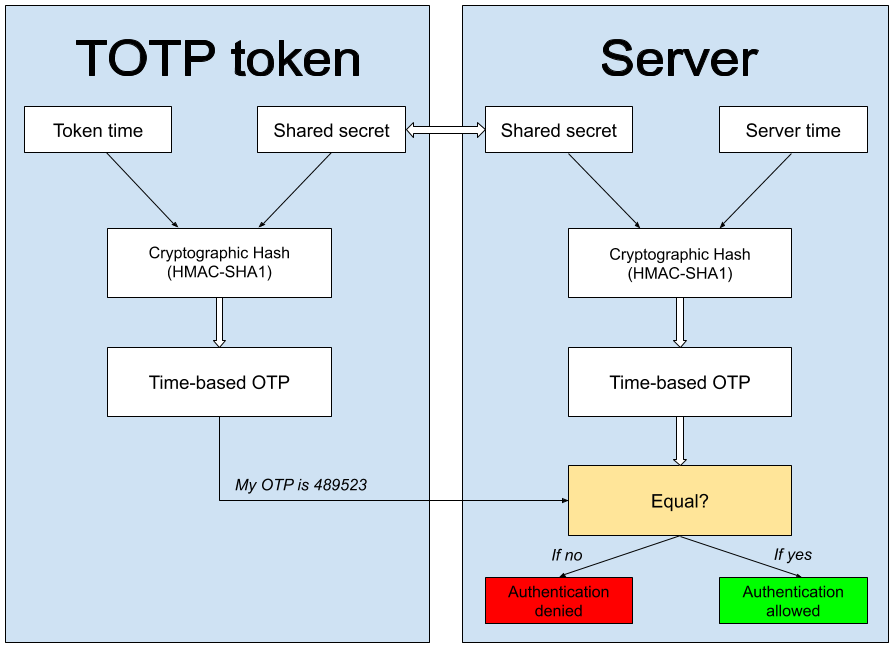
\includegraphics [width=15cm]{TOTP-algorithm-explained.png}
	\caption[Authentifikation durch TOTP]{Authentifikation durch TOTP}
	\label{fig:TOTP-algorithm-explained}
\end{figure}

Bei der timerbasierten (\ac{totp}) Methode wird die aktuelle Systemzeit (Token time) mit dem zu verschlüsselnden Text (Shared secret) anhand eines kryptografischen Verfahrens verschlüsselt. Es entsteht ein kryptografischer Hashwert (Cryptographic Hash), welcher meist den HMAC-SHA1 Hashingalgorithmus verwendet. Dieses Verfahren findet gleichermaßen auf dem Server statt. Der einzige Unterschied zum Server besteht darin, dass die Systemzeit des Servers genutzt wird. Findet innerhalb der festgelegten Zeit (ein Token entfällt laut RFC6238 standartmäßig nach 30 Sekunden, diese Zeit ist modifizierbar) eine erfolgreicher Match auf Serverseite statt, wird der User authentifiziert und ihm der Zugang gewährt. [13] Ein entscheidender Nachteil dieser Methode entsteht, falls der authentifizierende User innerhalb dieser 30 Sekunden (beispielsweise) durch eine Störung des Netzes oder einen kompletten Netzausfall die Verbindung verliert. Der aktuelle TOTP Code wird ungültig und muss erneut angefragt bzw. erstellt werden. Apps wie der Google Authenticator lösen dieses Problem, in dem sie einen Timer setzen und alle 30 Sekunden einen automatisch generierten neuen Code mit der aktuellen ablaufenden Zeit des Timers anzeigen. Dabei muss natürlich drauf geachtet werden, dass Server und Client synchron sind, dieses Verfahren ist deshalb an eine bestimmte Zeitspanne und ein externes Gerät (sei es Smartphone, TOTP Smart Card oder ein externer Rechner) gebunden. Diese Zeitbegrenzung bzw. das Verlassen auf die Zeit des Gerätes und des Servers kann zum Nachteil werden wenn Geräte asynchron werden. So gibt es einige ältere TOTP - Generatoren, die einen internen Zähler haben und mit jedem Tick eine Sekunde auf den aktuellen Wert nach UTC draufrechnen. Findet bei Geräterestart keine erneute Synchronisation (im RFC6238, Resynchronisation) statt, so entstehen fehlerhafte TOTP - Codes auf Clientseite, die der Server ablehnen wird. Dieser Nachteil ist gleichzeitig allerdings ein großer Vorteil in punkto Sicherheit, da ein Angreifer potenziell einen sehr kleinen zeitlich begrenzten Angriffsvektor besitzt, in dem er den TOTP - Code lösen muss. Durch entsprechende Zugriffssicherheitsfeatures, wie das Sperren des Nutzers nach oftmalig wiederholter falscher Eingabe, wird ein Bruteforce-Angriff verhindert.

Ereignisbasierte OTPs (folgend \ac{hotp}) besitzen einen Ereigniszähler, der bei jeder versuchten Authenzifizierung einen Zähler auf Server und Clientseite synchronisiert inkrementiert. Sollte der Zähler asychnron werden bzw. der Server einen anderen Wert gespeichert haben als der Client bei der nächsten Authentifizierung sendet, wird der Authentifizierungsvorgang abgebrochen. Man findet diese Funktionalität wortwörtlich beschrieben in Googles Time and event based one time password - Patent \cite{A6} in folgendem Wortlaut ``[...] the characteristics of an event can be the value of a counter that is incremented each time the user pushes a button on the token'' \cite{A6}. Für diesen Prozess wird ein spezieller Algorithmus genutzt, der im RFC4226 näher beschrieben ist.

Challenge-response basierte OTP Verfahren bedienen sich an komplizierten mathematischen Verfahren. Das heißt, es erfolgt ein ACK (Acknowledge bzw. Initialanstoß zur Authentifizierung). Der Client, berechnet die Response mithilfe der mathematischen Formel und sendet das Ergebnis an den Server. Sollte es einen Match geben, erhält der Client eine Response vom Server, der seine Echtheit bestätigt. Synchronisationsprobleme kann es bei diesem Verfahren entgegen der ereignis- oder timerbasierten OTP-Verfahren nicht geben, da die Berechnung dieses 'Schlüssels' vollkommen auf der Clientseite funktioniert. Der Server überprüft diese Rechnung nur mit seinem eigenen Wert, stellt aber keine weiteren Rechnungen oder Umformungen mit diesem Wert an. Der Hauptvorteil dieses Verfahrens ist, dass unabhängig von der Zeit und einem speziellen Ereignis eine Anfrage gestellt werden kann. Der Server kann also seine 'Challenge' abschicken und muss keine 'Response' innerhalb einer festgegebenen Zeit erhalten, um authentifizieren zu können. Dieses Verfahren gilt als besonders sicher, da es auf Serverseite keinen Algorithmus gibt, der sich vorausberechnen lässt.

Die folgende Tabelle soll vergleichend die Gemeinsamkeiten, aber auch Vor und Nachteile von HOTP mit TOTP verdeutlichen. Das Wissen zu vor allem den Nachteilen der Verfahren ist wichtig um die gewählte Eigenstrategie im Prototypen zu verstehen.

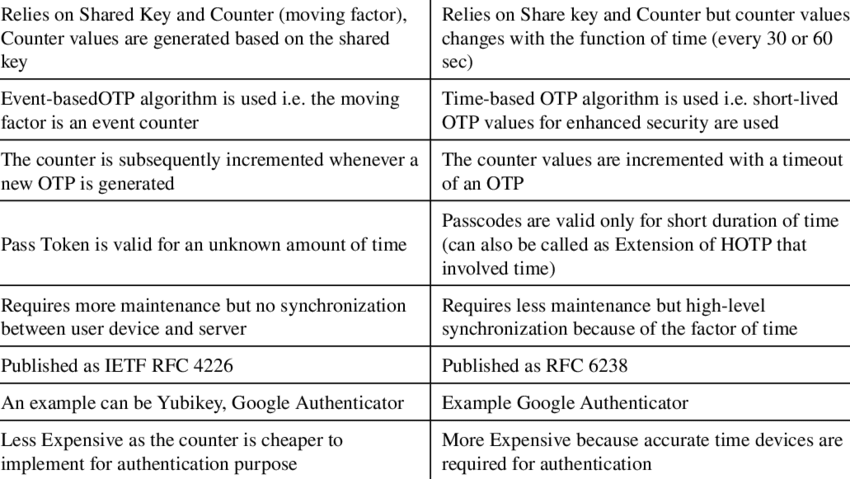
\includegraphics[width=15cm]{Tmp.png}
\newpage

\subsection{WebAuthn}
Webauthn ist kurz für die 'Web Authentication'. Zur Verfügung gestellt wurde dieser Standard der Authentifikation 2018 von der FIDO Alliance und dem W3C und ist vollumfänglich im FIDO2 Standard definiert. [A13] Sie ermöglicht eine passwortlose Authentifikation durch die Nutzung des vorhandenen public-key-Verfahrens für Webseiten.

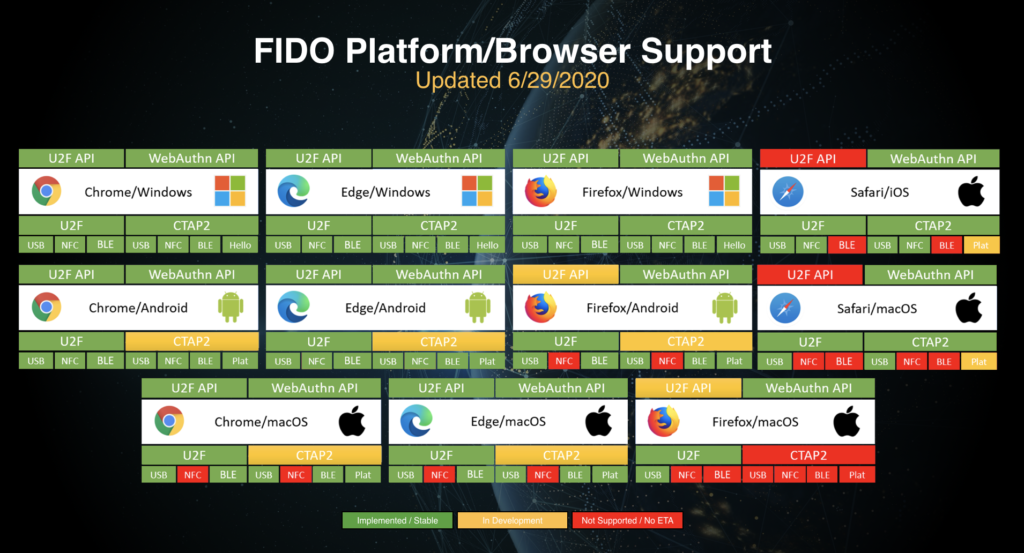
\includegraphics[width=15cm]{Screen-Shot-2020-06-30-at-8.11.50-AM-1024x553.png}

Die Abbildung von der FIDO - Alliance zeigt die Unterstützung von den FIDO - Ptorokollen, welche im vorangeggangenem Kapitel näher erläutert wurden. So besitzt zwar jeder Browser unter jedem Gerät die Unterstützung für die Webauthn API, allerdings unterstützt zum Beispiel der Browser 'Firefox' unter macOS das \ac{ctap}2 Protokoll nicht, welches somit die Untersützung der Webauthn API obsolet macht. Es sollte erwähnt werden, dass in der Abbildung ein gedanklicher Trennstrich zwischen den Beiden Paaren \ac{u2f}-API und \ac{u2f} sowie WebAuthn API und \ac{ctap}2 fehlt. Sie unterstützen sich nur als Paar gegenseitig allerdings nicht untereinander. Glieichzeitig bedeutet die Unterstützuing der \ac{ctap}2 Schnittstelle nicht automatisch, dass auch jede Variante der Authentifizierung möglich ist. So wird unter Windows unter den drei Browsern Google Chrome, Microsoft Edge und Firefox jede der vier Varianten unterstützt. Unter Android fehlt für alle drei Browser die Unterstützung von \ac{ctap}2. Unter macOS wiederrum wird \ac{ctap}2 im Safari-Browser unterstützt, doch NFC unf BLE zum Stand des Bildes (26.09.2020) nicht. Die Abbildung verdeutlicht, dass Webauthn zwar auf Geräten mit dem Windows - Betriebssystem vollumfänglich unterstützt werden, allerdings noch nicht zum allgemein implementierten Standard für andere Betriebssysteme geworden sind. So wie es ECMAScript6 (bzw. heutiges Javascript) oder Flash in jeden Browser geschafft hat. Dies ist ein Prozess und wird wohl noch einige Jahre andauern, bis alle Browser die \ac{ctap}2 Schnittstelle unterstützen und damit eine Webauthn - Authentifizierung ermöglichen.

Der Standard definiert verschiedene Arten von Authentifikationsmöglichkeiten. Neben sogenannten ``plattform authenticators`` [13] also jenen Verfahren, die die geräteeigenen Sicherheitsfeatures wie den Fingerabdrucksensor oder der Gesichtserkennung durch eine Kamera nutzen, definiert der Standard auch die Authentifizierung durch externe Geräte wie USB-Sticks, auf denen sich der private Schlüssel des Nutzers (in gesicherter Form) befindet. Grundsätzlich definiert WebAuthn nur Dinge, die man im nativen Bereich bereits kennt, adaptiert diese allerdings für den Webbereich. Dabei basiert Webauthn auf vielen bereits vorhandenen Abhängigkeiten der Informatik wie die Standards von HTML5, ECMAScript, COSE (CBOR Object Signing and Encryption COSE, definiert im RFC8152) oder dem Nutzen von der Base64url encoding.

Laut dem W3C sei die grundsätzliche Idee hinter diesem Verfahren, dass die Daten des Users zu keinem Zeitpunkt den Rechner verlassen müssen. Die Daten werden vollumfänglich vom jeweiligen Authenticator gemanaged, welches dann mit einer sogenannten 'Relying Party' interagiert um den Nutzer zu authentifizieren. Eine Relying Party ist grob vereinfacht eine Entität, welche die Web Authentication API nutzt um den Nutzer zunächst einmal zu registrieren und in Zukunft zu authentifizieren. [13]

Auf einer von Codegram organisierten Rede von Suby Raman, einem der Mitentwickler des Web-Authentication-Protokolls und dem Hauptentwickler für Windows Hello, erläutert Raman die Probleme von Passwörtern, die im Rahmen dieser Arbeit im Kapitel der Einleitung bereits addressiert worden, und wie WebAuthn diese löst.

\begin{enumerate} 
\item \textbf{Passwörter sind geteilte Geheimnisse.}

Der ausgetauschte öffentliche Schlüssel ist kein Geheimnis, der private Schlüssel bleibt stets auf dem Gerät des Nutzers und verlässt diesen zu keinem Zeitpunkt der Authentifikation.

\item \textbf{Sichere Passwörter sind schwer zu finden und wenn, dann sind sie nicht leicht merkbar.}

Der Authenticator auf den Geräten des Nutzers erstellt zufällige und sichere 'credentials' für die Authentifikation. Es liegt nicht mehr in der Verantwortung des Nutzers dies zu tun.

\item \textbf{Passwörter können leicht entwendet werden.}

Sichere interne (oder auch externe) Hardware macht es Angreifern sehr schwer, wenn nicht schon fast mathematisch unmöglich, durch physische Angriffe an die privaten Schlüssel zu kommen. Zum Verfassungszeitpunkt dieser Arbeie sind keine Angriffe auf diese Geräte bekannt, vereinzelt gibt es dennoch Angriffe auf die Software der Hersteller, die sich auf den Geräten vorinstalliert befindet.

\item \textbf{Passwörter haben ein Bequemlichkeitsproblem und sorgen automatisch für die unsichere Wahl dessen.}

Die 'credentials' des Nutzers sind gebunden an den aktuellen Scope des Nutzers. Das heißt das jede Anfrage einzigartig ist. Dies gillt sowohl für die Registrierung als auch den späteren Login mithilfe der Web Authentication API. Der erwähnte Wiederholungsangriff im Kapitel für Unsichere Passwörter wird damit verhindert. Ein mehrmaliges Nutzen der erstellten zufälligen Daten durch den Authenticator ist damit nicht möglich und nur für eine Anfrage valide.

\item \textbf{Aus Sicht der Entwickler sind Passwörter schwer zu sichern.}

Da der öffentliche Schlüssel kein Geheimnis darstellt, hat dieser auch keinen besonderen Wert und kann problemlos im Klartext in Datenbanken persistiert werden.
\end{enumerate}

Zusammengefasst hat der FIDO2 Standard mit \ac{ctap} (dem Protokoll für externe Authentifikationen mit Mobilgeräten) und Webauthn (der Schnittstelle bzw. ''API``) vorhandene Funktionen definiert, mit der native Authentifizierungsmethoden wie das public-private Key Verfahren auf die Webseite übertragen werden können.
